 \documentclass{beamer}
%   \documentclass[handout]{beamer}
%\beamertemplatenavigationsymbolsempty
%\setbeamertemplate{footline}[frame number]

\usepackage[ansinew,latin1]{inputenc}
%\usepackage[T1]{fontenc}
%\usepackage[latin1]{inputenc}
%\usepackage[utopia]{mathdesign}
%\usepackage[english]{babel}
\usepackage{amsmath,amsfonts,amssymb,amsthm}
\usepackage{mathtools}
\usepackage{commath}
\usepackage{multirow}
\usepackage{booktabs}
\usepackage{tikz}
\usepackage{tikz-qtree}
\usetikzlibrary{trees}
\newcommand\MyBox[2]{
	\fbox{\lower0.75cm
		\vbox to 1cm{\vfil
			\hbox to 2cm{\hfil\parbox{1cm}{#1\\#2}\hfil}
			\vfil}%
	}%
}

%\usepackage{beamerthemesplit}
%\usepackage{beamertemplates}
%\beamertemplatetransparentcovereddynamic

% packages

\usepackage{amsmath}
\usepackage{tcolorbox}
\usepackage{amscd}
\usepackage{amsxtra}
\usepackage{delarray}
\usepackage{alltt}
\usepackage{eurosym}
\usepackage{blkarray}


%\textheight9cm \textwidth13cm

\newcommand{\var}{\mbox{\rm Var}}
\newcommand{\cov}{\mbox{\rm Cov}}       % für Formeln
\newcommand{\cor}{\mbox{\rm Corr}}      % für Formeln
\newcommand{\e}{\mbox{E}}               % für Formeln
\newcommand{\p}{\mbox{P}}               % für Formeln
\newcommand{\diag}{\mbox{\rm diag}}
\newcommand{\spur}{\mbox{\rm spur}}
\newcommand{\D}{\displaystyle}
\newcommand{\s}{\scriptsize}
\newcommand{\ve}[1]{\mbox{$\boldsymbol{#1}$}}
\newcommand{\ma}[1]{\mbox{$\mathbf{#1}$}}
\newcommand{\gma}[1]{\mbox{$\boldsymbol{#1}$}}

\newcommand{\suba}{{\text{\scriptsize \ma{a}}}}
\newcommand{\subb}{{\text{\scriptsize \ma{b}}}}
\newcommand{\subc}{{\text{\scriptsize \ma{c}}}}
\newcommand{\sube}{{\text{\scriptsize \ma{e}}}}
\newcommand{\subf}{{\text{\scriptsize \ve{f}}}}
\newcommand{\subu}{{\text{\scriptsize \ma{u}}}}
\newcommand{\subx}{{\text{\scriptsize \ve{x}}}}
\newcommand{\suby}{{\text{\scriptsize \ve{y}}}}
\newcommand{\subz}{{\text{\scriptsize \ve{z}}}}
\newcommand{\subA}{{\text{\scriptsize \ma{A}}}}
\newcommand{\subB}{{\text{\scriptsize \ma{B}}}}
\newcommand{\subI}{{\text{\scriptsize \ma{I}}}}
\newcommand{\subT}{{\text{\scriptsize \ma{T}}}}
\newcommand{\subX}{{\text{\scriptsize \ma{X}}}}
\newcommand{\subxi}{{\text{\scriptsize \ve{\xi}}}}
\newcommand{\subbeta}{{\text{\scriptsize \ve{\beta}}}}
\newcommand{\subdelta}{{\text{\scriptsize \ve{\delta}}}}
\newcommand{\subeta}{{\text{\scriptsize \ve{\eta}}}}
\newcommand{\subzeta}{{\text{\scriptsize \ve{\zeta}}}}
\newcommand{\subeps}{{\text{\scriptsize \ve{\varepsilon}}}}
\newcommand{\subbeob}{{\text{\scriptsize \it beob}}}
\newcommand{\subfehl}{{\text{\scriptsize \it fehl}}}
\newcommand{\subvoll}{{\text{\scriptsize \it voll}}}
\newcommand{\subred}{{\text{\scriptsize \it reduziert}}}
\newcommand{\sbullet}{\text{{\scriptsize $\bullet$}}}

\newcommand{\R}{\mathbb{R}}
\newcommand{\Z}{\mathbb{Z}}
\newcommand{\mycolorbox}[1]{\colorbox{blue}{\begin{minipage}{18.5cm}#1 \end{minipage}} }

\newcommand{\eq}{\mbox{\raisebox{.5pt}{\footnotesize$\,=\,$}}}
\newfont{\cmsy}{cmsy10.tfm}
\newcommand{\gauklam}[1]{\mbox{\cmsy{\symbol{98}}} #1 \mbox{\cmsy{\symbol{99}}}}
\newcommand{\BS}{\mbox{\cmsy{\symbol{110}}}}
\newcommand{\HK}{\symbol{34}}
\newcommand{\mycbox}[1]{\colorbox[gray]{0.85}{#1}}

\newcommand{\inpic}[1]{\input{d:/vorles/multvorl/bilder/#1}}

\definecolor{darkgreen}{cmyk}{0.7,0,0.2,0.7}

\definecolor{grau}{gray}{0.25}
\definecolor{dkgreen}{rgb}{0,0.6,0}
\definecolor{darkblue}{rgb}{0,.1,.4}
\definecolor{lightblue}{RGB}{176,194,255}
\definecolor{lightgreen}{RGB}{184,255,176}
\definecolor{orange}{rgb}{1,0.5,0}
\definecolor{lgray}{gray}{0.95}
\definecolor{dkblue}{RGB}{0, 51, 102}
\def\bs{\boldsymbol}
\newcommand{\code}[1]{\texttt{#1}}

%\input{R-listings}
\usepackage{mathrsfs}
\usepackage{epsfig}
\usepackage{textcomp}



% Für Handouts
%\usepackage{pgfpages}
%\pgfpagesuselayout{2 on 1}[a4paper,border shrink=5mm]

% Makros
\def\med{\mathop{\rm med}}
\def\var{\mathop{\rm var}}
\def\sign{\mathop{\rm sign}}
\newcommand{\adist}{\sim \hspace{-0.20cm}:\hspace{0.17cm}}

\newenvironment{liste}{\begin{list}{-}{ \setlength{\itemsep}{0cm}
\setlength{\topsep}{0cm} \setlength{\parsep}{0cm} \setlength{\parskip}{0cm}}}{\end{list}}

\newenvironment{abcliste}{\begin{list}{\alph{enumi})}{\usecounter{enumi}
\setlength{\itemsep}{0cm} \setlength{\topsep}{0cm} \setlength{\parsep}{0cm} \setlength{\parskip}{0cm}}}{\end{list}}

\newenvironment{123liste}{\begin{list}{\arabic{enumi})}{\usecounter{enumi}
\setlength{\itemsep}{0cm} \setlength{\topsep}{0cm} \setlength{\parsep}{0cm} \setlength{\parskip}{0cm}}}{\end{list}}



% Einstellungen fürs Layout
\usetheme[headheight=0mm, footheight=3mm]{boxes}
\usecolortheme{dolphin}
\useinnertheme{circles}
\useoutertheme{infolines}
\beamertemplatenavigationsymbolsempty
%\beamertemplatetransparentcovereddynamic

% Farben definieren...
\newcommand{\pkg}[1]{{\fontseries{b}\selectfont #1}}
\def\cola{\usebeamercolor[fg]{example text}}
\setbeamercolor{beamer red}{fg=red}
\def\colb{\usebeamercolor[fg]{beamer red}}
\def\colc{\usebeamercolor[fg]{titlelike}}
\definecolor{text-grey}{rgb}{0.45, 0.45, 0.45} % grey text on white background
\definecolor{bg-grey}{rgb}{0.66, 0.65, 0.60} % grey background (for white text)
\definecolor{fu-blue}{RGB}{0, 51, 102} % blue text
\definecolor{fu-green}{RGB}{153, 204, 0} % green text
\definecolor{fu-red}{RGB}{204, 0, 0} % red text (used by \alert)

\title[Statistical Machine Learning]{STAT380 \\Statistical Machine Learning}
\author[STAT380]{Department of Analytics in the Digital Era\\Collegue of Business and Economics\\United Arab Emirates University}
\institute[]{}
\date[UAEU]{}


\addtolength{\textheight}{0.2in}
\setlength{\itemsep}{-0.2ex minus0.2ex}
\setlength{\parsep}{0ex minus0.2ex}
%\setlength{\mathindent}{0cm}
\setlength{\jot}{2ex}
\setlength{\topsep}{0ex plus0.5ex minus0.2ex}





\begin{document}

%\include{chapter/syllabus}

\section{Introduction}



\begin{frame}{Outlook of the unit}
	
	\begin{itemize}
		\item[3] \textbf{Prediction and classification approaches}
		\vspace{0.2cm}
	\begin{itemize}

		\item Classifiers
			\begin{itemize}
			\item Logistic regression
				\vspace{0.2cm}
			\item Discriminant analysis
					\end{itemize}
			\vspace{0.2cm}
			\item Classifier performance
				\vspace{0.2cm}
			\item Tree-based methods: Decision trees
				\vspace{0.2cm}
				\begin{itemize}
				\item Classification trees
				\vspace{0.2cm}
				\item
				Regression trees
	\end{itemize}
		\end{itemize}
		\end{itemize}		
\end{frame}


\begin{frame}
	\begin{center}
		\Large{\textcolor{dkblue}{Classifiers}}
	\end{center}
\end{frame}

\begin{frame}
	\begin{figure}	
		\frametitle{Prediction and classification approaches - A short overview}
		\centering
		\hspace*{-0.8cm}
		%\includegraphics[width=0.96\textwidth]{bilder/Process} \\
	\end{figure}
\end{frame}



%---------------------------------------------

\begin{frame}
	\frametitle{Examples of classification}
	
	\begin{itemize}
		\item Banking: determining whether a transaction is fraudulent or an 
		applicant is a good or bad credit risk.
			\vspace{0.2cm}
		\item E-commerce: forecasting whether a particular order will be paid 
		for or which customer will buy a specific product.
			\vspace{0.2cm}
		\item National security: identifying whether a certain behavior 
		indicates a possible thread.
			\vspace{0.2cm}
		\item Tourism: determining the rating a hotel should be awarded.
			\vspace{0.2cm}
		\item Medicine: diagnosing whether a particular disease is present.
		
		\vspace{0.3cm}
		
	\end{itemize}
\end{frame}


\begin{frame}
	\frametitle{Assumptions}
	

	\begin{itemize}
		\item Extracting knowledge from massive data sets assumes that they contain non-random, useful information.
			\vspace{0.2cm}
		\item Classification algorithms, especially predictions, do not have further assumptions about how the data was generated.
			\vspace{0.2cm}
		\item Most classical statistical methods are not valid if their \textbf{assumptions} are not fulfilled.
	\end{itemize}
	\vspace{0.8cm}
	This does not mean that big data is always good data.
	
\end{frame}

\begin{frame}
	\frametitle{Definition: Basics}
	
	$n$ number of observations in a sample
	
	$p$ number of predictor variables (features)
	
	\vspace{0.5cm}
	
	$X = \left(
	\begin{matrix}
		x_{11} & x_{12} & \cdots & x_{1p} \\
		x_{21} & x_{22} & \cdots & x_{2p} \\
		\vdots & \vdots & \ddots & \vdots \\
		x_{n1} & x_{n2} & \cdots & x_{np}
	\end{matrix} 
	\right)$
	\small{matrix of predictor variables}
	
	\hspace{0.5cm}	
	
	$y = \left(
	\begin{matrix}
		y_1  \\
		y_2  \\
		\vdots  \\
		y_n 
	\end{matrix} 
	\right)$  
	\small{vector of response (dependent / target) variable}
	
	\hspace{0.5cm}
	
	$\{(x_1, y_1), (x_2, y_2), \cdots, (x_n, y_n) \}$, where $x_i$ is a vector of 
	length $p$, represents the observed data from which 
	a statistical model is built. 			
\end{frame}



\begin{frame}
	\frametitle{Definition: Classification}
	
	Classification employs a set of $p$ inputs to explain a value of an outcome 
	variable $y$.
		\vspace{0.2cm}
	\begin{itemize}
		\item $x$ is an object in an object space $\mathbb{X}$	
		\vspace{0.2cm}
		\item $y = y(x)$ is the response in a response space $\mathbb{Y}$
			\vspace{0.2cm}
		\item Algorithm $a(x)$ is a function from $\mathbb{X}$ to $\mathbb{Y}$
	\end{itemize}
	
	
	
	
	
	
	
	\vspace{0.3cm}
	
	In classification, $\mathbb{Y}$ is a set of discrete categories, $\{C_1, C_2, 
	..., 
	C_K\}$, exclusively and exhaustively defining possible states of an element.
		\vspace{0.2cm}
	$\mathbb{Y} = \{C_1, C_2\}$ binary classification
	
	$\mathbb{Y} = \{C_1, C_2, ..., C_K\}$ multiclass classification
	
\end{frame}





\begin{frame}
	\frametitle{Place of classification among other methods}
	
	\begin{itemize}
		
		\item Classification is a method of supervised learning for a \textbf{categorical} 
		output
			\vspace{0.2cm}
		\item If $y$ is continuous: it is a regression problem (also supervised learning)
			\vspace{0.2cm}
		
		\item If categories $C_k$ are not defined: unsupervised learning (e.g. 
		clustering) 	
	\end{itemize}
\end{frame}



\begin{frame}
	\frametitle{Process of generating and using a model: remember}
	
\textbf{	Step 1: training a model}
		\vspace{0.2cm}
	Historical data is used to generate a statistical model that predicts a 
	response variable from a set of predictor variables
	
	\vspace{0.5cm}
	
\textbf{	Step 2: deploying a model}
		\vspace{0.2cm}
	Predictions for the response variables for a new data set with the same 
	predictor variables are made		
\end{frame}




\begin{frame}
	\frametitle{Training model: Major decisions}
	
	Given a real-world problem and data you need to decide on:
	\begin{enumerate}
		\item which classifier to use
			\vspace{0.2cm}
		\item which features to take from the data
			\vspace{0.2cm}
		\item which evaluation metric to optimize 
	\end{enumerate}
\end{frame}

\note[enumerate]{ 
	\item To the 2nd: the tree methods we discuss in this section offer implicit variable selection, next session on regression also presents a way to choose the most important predictors  
	\item To the 3rd: one can rely on statistical metrics or be more business oriented and e.g. assign costs to different correct and erroneous predictions}

\subsubsection{Choose Classifier}

\begin{frame}
	\frametitle{Large 'Zoo' of Classification Methods}
	
	Classifiers differ by: 
	
	\begin{itemize}
		\item ways to construct decision boundary (linear vs. non-linear).
			\vspace{0.2cm}
		\item types of data they can use as inputs.
			\vspace{0.2cm}
		\item probabilities to be a member of a particular class or only class 
		membership is predicted.
			\vspace{0.2cm}
		\item number of times a model is built (individual vs. ensemble).
	\end{itemize}
\end{frame}

\note{relate to disciminant analysis that participants can be familiar with} %ToDo



\begin{frame}
	\frametitle{Constraints}
	Decision of which classifier to use is subject to constrains:
	\begin{itemize}
		\item analyst's understanding of algorithms
		\vspace{0.2cm}
		\item interpretability
		\vspace{0.2cm}
		\item runtime
		\vspace{0.2cm}
		\item scalability
	\end{itemize}
\end{frame}







\subsubsection{Evaluate Performance}







\subsection{Logistic regression}

\begin{frame}
	\begin{center}
		\Large{\textcolor{dkblue}{Logistic regression}}
	\end{center}
\end{frame}



\begin{frame}{What is meant by binary logistic regression analysis?}
	\vspace{-3mm}
	In the previous lectures, you learned the basic concepts of the\textbf{ linear regression model and their estimation}.\\
	\vspace{3mm}
	Why do we need additional regression methods?
	\vspace{3mm}
	\begin{itemize}
		\item Previously worked with the predictions continuous target variables. 
		\vspace{3mm}
		\item What can we use to explain categorical variables?
		\vspace{3mm}
		\item[$\rightarrow$] \textbf{target}: Model a dependent \textbf{binary variable} to make an appropriate prediction of probability (using covariates).
\end{itemize}
\end{frame}		


\begin{frame}{Examples of binary variables}
	\vspace{-7mm}
Let's imagine independent observations $y_1,\ldots,y_n$ of a
	variable of interest $Y$, which can take \textbf{only two values} (e.g. 0 and 1), e.g.:
	\vspace{3mm}
	\begin{itemize}
		\item Workpiece is defective(1)/not defective(0)
		\vspace{3mm}
		\item Customer is considered creditworthy: yes(1)/no(0)
		\vspace{3mm}
		\item Therapy is successful: yes(1)/no(0).
	\end{itemize}
	\vspace{3mm}
	$\rightarrow$ Is linear regression \textbf{optimal} for modeling binary dependent variables?
\end{frame}


\begin{frame}{Illustration: UAE funding award to high schools }
	\vspace{-3mm}
	\begin{itemize}
		\item  This award is given for the best high school graduation performance in AL Ain.
		\vspace{3mm}
		\item
		What is the probability of receiving this price, depending on the hours of literature the high school graduates have read in the last year?
		\vspace{3mm}
		\item
		The variable \textit{Award} is coded 0 if the person did not win the prize and 1 if the person won the prize.
	\end{itemize}
\end{frame}

\begin{frame}
	\begin{figure}	
		\frametitle{Illustration: UAE funding award}
		\centering
		\hspace*{-0.8cm}
		%\includegraphics[width=0.6\textwidth]{bilder/award} \\
	\end{figure}
\end{frame}


\begin{frame}
	\begin{figure}	
		\frametitle{Illustration: Prediction of probabilities?}
		\centering
		\hspace*{-0.8cm}
		%\includegraphics[width=0.6\textwidth]{bilder/bi} \\
	\end{figure}
\end{frame}

\begin{frame}
	\begin{figure}	
		\frametitle{Illustration: Model assumptions}
		\centering
		\hspace*{-0.8cm}
		%\includegraphics[width=0.6\textwidth]{bilder/resibi} \\
	\end{figure}
\end{frame}

\begin{frame}{Problems with linear regression}
	\vspace{-9mm}
	\begin{itemize}
		\item Insufficient spread: residuals do not spread uniformly; clear systematic spread
		\vspace{3mm}
		\item Violation of normal distribution assumption: residuals must be normally distributed; this is clearly not the case here
		\vspace{3mm}
		\item Variance homogeneity not fulfilled
		\vspace{3mm}
		\item Implausible values for modeling a probability in the estimation results: Values $<0$ and $>1$
	\end{itemize}
	\vspace{3mm}
	$\rightarrow$ \textbf{Binary logistic regression analysis}
\end{frame}


\begin{frame}{Modeling the influence of explanatory variables}
	\vspace{-3mm}
	\begin{itemize}
		\item A distribution model for binary target variables $Y_i$ is the binomial distribution, $Y_i \sim B(1,\pi_i)$ with $\text{Var}(Y_i)=\pi_i(1-\pi_i) $ and $\pi_i=P(Y_i=1)=E(Y_i)$.
		\vspace{2mm}
		\item In what follows, we will call one of the two possible values of Y a
		success and the other as a failure.
		\vspace{2mm}
		\item We call $\pi_i$ as the probability of success.\
		\vspace{2mm}
		\item \textbf{Target}: Given p explanatory variables: $x_1,\ldots,x_p$, we model the influence of the explanatory variables on
		$\pi_i$.
		\begin{itemize}
			\vspace{2mm}
			\item[-] How does the probability of a customer repaying their
			loan repaid as a function of the customer's age?
		\end{itemize}
	\end{itemize}
	
\end{frame}

\begin{frame}
	\begin{figure}	
		\frametitle{Illustration: Prediction of probabilities!}
		\centering
		\hspace*{-0.8cm}
		%\includegraphics[width=0.6\textwidth]{bilder/bibi} \\
	\end{figure}
\end{frame}

\begin{frame}

				\frametitle{Logistic regression definition}

		This model is used to fit a relationship between a categorical outcome variable $\textbf{y}$ (for instance: binary 0-1) and a set of predictors (covariates) $\textbf{X}$:\\[2mm]
		\textbf{Response/ Mean function:}
		\begin{align}\nonumber
			\pi_i=P(Y_i=1\,|\,\ve{x}_i'\ve{\beta})=F(\eta_i)=\frac{\exp{(\eta_i)}}{1 + \exp{(\eta_i)}}
		\end{align}
		\textbf{Link function:}
		\begin{align}\nonumber
			g(\pi_i)=\log\left(\frac{\pi_i}{1-\pi_i}\right)=\eta_i = \ve{x}_i' \ve{\beta},
		\end{align}
		where $\eta_i=\ve{x}_i' \ve{\beta}$ denotes the linear predictor.

		
		

\end{frame}


\begin{frame}{Odds ratio}
	\vspace{-3mm}
	$\rightarrow$ The probability $\pi_i$ is transformed to $odds_i$ :\\
	\vspace{2mm}
	Closely related to the probability of an event occurring is the notion of \textbf{chance (odds-ratio)}.
	\vspace{2mm}
	\begin{itemize}
		\item It denotes the ratio between the probability of success and the failure probability.
		$$Odds_i:=\frac{P(Y_i=1)}{P(Y_i=0)}=\frac{P(Y_i=1)}{1-P(Y_i=1)}=\frac{\pi_i}{1-\pi_i}$$
		\item Example: If the odds in favor of success (winning) of a
		racer are 20:1, then we \emph{expect} him to win 20 and lose one out of 21
		20 games and lose one.
	\end{itemize}
\end{frame}

\begin{frame}{Global interpretation of coefficients}
	\vspace{-3mm}
\begin{itemize}
	\item Since the marginal effects are not constant, the coefficients $\hat{{\beta}}$ can be
	poorly interpreted directly.
	\vspace{3mm}
	\item
	Instead, one usually interprets $\exp(\hat{{\beta}})$.
\end{itemize}
\begin{table}[ht]
	\centering
	\begin{tabular}{ccc}
	\hline
coefficient $\hat{{\beta}}$ & chance $\frac{P(Y_i = 1)}{P(Y_i = 0)}$ & probability $P(Y_i = 1)$\\ 
	\hline
$\hat{{\beta}}> 0$ & increases by $\exp(\hat{{\beta}})$ & increases \\ 
$\hat{{\beta}}< 0$ & decreases by $\exp(\hat{{\beta}})$ & decreases \\ 
$\hat{{\beta}} = 0$ & remains the same & remains the same \\
	\hline
	\end{tabular}
\end{table}



\end{frame}


\begin{frame}{Illustration: interpretation of results}
	\vspace{-3mm}
\begin{itemize}
		\item 
	Model to be estimated: $\frac{\exp{(\beta_0 + \beta_1*Read)}}{1 + \exp{(\beta_0 + \beta_1*Read)}}$
		\vspace{0.2cm}
	\item Estimated parameters: $\hat{{\beta_0}}=-9.8$ and $\hat{{\beta_1}}=0.16$
		\vspace{0.2cm}	
	
	\item [$\rightarrow$] $\exp(0.16) = 1.169$: The chance that a student will win the prize given an increase of
	of the lessentime by one hour is valid, averaged by 1.169 times higher.
	\vspace{0.2cm}	
	\item [$\rightarrow$] $\frac{\exp{(-9.8+0.16*70)}}{1 + \exp{(-9.8+0.16*70)}}=0.8$: The probability with which a
	a student, who reads 70 hours in the final year of school will win the prize.
		\vspace{0.2cm}	
	\item [$\rightarrow$] $Odds_{1(70)}:=\frac{\pi_{1(70)}}{1-\pi_{1(70)}}=4$: The student
	(Observation i=1) who reads 70 hours has a 4 times higher chances of
 winning the prize than  not winning it.
\vspace{0.2cm}	
\item
The constant parameter cannot be interpreted meaningfully.
\end{itemize}
\end{frame}


\subsection{Linear discriminant analysis}

\begin{frame}
	\begin{center}
		\Large{\textcolor{dkblue}{Linear discriminant analysis}}
	\end{center}
\end{frame}


\begin{frame}{Discriminant analysis}
	\begin{itemize}
		\item
		In case the response variable contains \textbf{more than two categories}, discriminant analysis is more suitable than the logistic regression.
		\vspace{0.2cm}	
		\item
		It predicts the probability of belonging to a given category based on explanatory variables.
		\vspace{0.2cm}	
	\end{itemize}
\end{frame}


\begin{frame}{\textbf{Why do we need another method, when we have logistic regression?}}
	\begin{itemize}
		\item
		When the classes are well-separated, the parameter estimates for the
logistic regression model are surprisingly \textbf{unstable}. Linear discriminant
analysis does not suffer from this problem.
	\vspace{0.2cm}	  
		\item
		linear discriminant analysis is popular
when we have more than two response classes.
		\vspace{0.2cm}	
		\item
		If \textbf{$n$ is small} and the distribution of the predictors $X$ is approximately
normal in each of the classes, the linear discriminant model is again
more stable than the logistic regression model.
	\end{itemize}
\end{frame}


\begin{frame}{Linear Discriminant analysis: ideas behind}
	\begin{itemize}
	\item
	Logistic regression involves directly modeling $Pr(Y = k|X = x)$ using the
	logistic function, for the case of two response classes. 
	\vspace{0.2cm}	  
	\item
	Commonly, we model the conditional distribution of the response $Y$ ,
	given the predictor(s) $X$. 
	\vspace{0.2cm}	  
	\item
	We now consider an \textbf{alternative} and less direct
	approach to estimating these probabilities. 

	\vspace{0.2cm}	  
\item
In this alternative approach,
we model the \textbf{distribution} of the predictors $X$ separately in each of the
response classes (i.e. given $Y$ ), and then use\textbf{ Bayes' theorem} to flip these
around into estimates for $Pr(Y = k|X = x)$. 
\vspace{0.2cm}	  
\item
When these distributions are
assumed to be normal, it turns out that the model is very similar in form
to logistic regression.
\end{itemize}
\end{frame}


\begin{frame}{Linear discriminant analysis: ideas behind}
	\begin{itemize}
		\item
		\textbf{L}inear \textbf{D}iscriminant \textbf{A}nalysis (\textbf{LDA}) is an alternative to the logistic regression.
				\vspace{0.2cm}	
		\item
		It helps to find the \textbf{linear combination }of predictors that provide the best possible separation between the groups.
		\vspace{0.2cm}	
		\item
		It this data to divide the space of covariates into regions. The regions are labeled by categories and have \textbf{linear boundaries} (L in LDA).	
	\vspace{0.2cm}	
		\item
		Those boundaries are a consequence of assuming that the covariates for each category have the same \textbf{multivariate normal distribution}.
	\end{itemize}
\end{frame}


\begin{frame}{Bayes classifier}
	\begin{itemize}
		\item
	It	assigns each observation to the most likely class,
given its predictor values.
		\vspace{0.2cm}	
		\item
		In a two-class problem where there are only two possible response values, say class 1 or class 2, the Bayes classifier corresponds to predicting class one if $Pr(Y = 1|X = x0) > 0.5$, and class
two otherwise.	
	\vspace{0.2cm}	
\item
Bayes theorem for classification:
	\begin{align*}\nonumber
	Pr(Y=k|X=x)&=\frac{Pr(Y=k|X=x)Pr(Y=k)}{Pr(Y=k)}\\
	&=\frac{\pi_kf_k(x)}{\sum_{l=1}^{k}(\pi_lf_l(x))}
\end{align*}	
	\end{itemize}
\end{frame}


\begin{frame}[fragile]{Discriminant analysis: Boston housing data}
With the {lda()}-command we can perform a lda
	\begin{lstlisting}
# Discriminant analysis 
linear <- lda(CAT..MEDV~., train)
linear
p <- predict(linear, train)
ldahist(data = p$x[,1], g = train$CAT..MEDV)

# Discriminant analysis density plots
sm.lda <- lda(CAT..MEDV~., train)
print(sm.lda)
p<- predict(sm.lda, train)
p.df <- data.frame(LD1 = p$x, class = p$class) 
print(p.df)
lggplot(p.df) + geom_density(aes(LD1, fill = class), alpha = 0.2)		
	\end{lstlisting}
		
\end{frame}


\begin{frame}[fragile]{Stacked histogram for discriminant function values: Boston housing data}
	\begin{center}
		\includegraphics[width=0.8\textwidth]{bilder/lda1}
	\end{center}	
\end{frame}

\begin{frame}[fragile]{Density plots from discriminant analysis: Boston housing data}
	\begin{center}
		\includegraphics[width=0.8\textwidth]{bilder/lda2}
	\end{center}	
\end{frame}

\subsection{Classifier performance}

\begin{frame}
	\begin{center}
		\Large{\textcolor{dkblue}{Classifier performance }}
	\end{center}
\end{frame}








\begin{frame}
\frametitle{Judging classifier performance}
\textbf{Some first comments}:\\
\begin{itemize}
  \item A natural criterion for judging the performance of a classifier is the probability
of making a \textbf{misclassification} error.
\vspace{0.2cm}
\item Misclassification means that the record
belongs to one class but the model classifies it as a member of a different class.
\vspace{0.2cm}
\item A classifier that makes no errors would be perfect - unrealistic.
\vspace{0.2cm}
\item Is there a minimal
probability of misclassification that we should require of a classifier?
\end{itemize}
\end{frame}


\begin{frame}
\frametitle{Misclassification error}
\begin{figure}
	\centering
	\includegraphics[width = 8cm]{bilder/eroor.png}
\end{figure}
\end{frame}


\begin{frame}
\frametitle{Benchmark: The naive rule}
\begin{itemize}
  \item A very simple rule for classifying a record into one of $m$ classes, ignoring all predictor
information is to classify the record
as a member of the \textbf{majority class}.
\vspace{0.2cm}
\item The \textbf{naive rule} is used mainly as a baseline or benchmark
for evaluating the performance of more complicated classifiers.
\vspace{0.2cm}
\item Similar to using to $\overline{y}$ as the naive benchmark in the numerical
outcome case, the naive rule for classification relies solely on the $y$ information
and excludes any additional predictor information.
\vspace{0.2cm}
\item A good classifier
that uses external predictor information should outperform the naive rule.
\end{itemize}
\end{frame}

\begin{frame}
\frametitle{A more complex approach: Logistic regression}
A popular model for making classifications is the logistic regression
model. To predict which class a
new record $\textbf{x}_i$ will belong to we compute its probability to belong to each class by
\begin{align}\nonumber
\hat{\pi}_i=\frac{\exp{(\hat{\eta}_i)}}{1 + \exp{(\hat{\eta}_i)}}=\frac{\exp{(\ve{x}_i' \ve{\hat{\beta}})}}{1 + \exp{(\ve{x}_i' \ve{\hat{\beta}})}}
\end{align}
and then
possibly rank a set of new records from highest to lowest probability in order to
act on those with the highest probability.
\end{frame}

\begin{frame}
\frametitle{Accuracy measures - the classification matrix}
\begin{itemize}
  \item Classification matrix summarizes the correct and incorrect classifications
that a classifier produced.
  \item Rows and columns
of the confusion matrix correspond to the predicted and true (actual) classes.
\item Example:\\[-2mm]
\begin{tabular}{cccc}

  % after \\: \hline or \cline{col1-col2} \cline{col3-col4} ...
 &  & \multicolumn{2}{|l}{Actual class} \\
  & & \multicolumn{1}{|c}{0} & 1 \\\hline
\multirow{2}{*}{Predicted class} & 0 & \multicolumn{1}{|c}{2600} & 100 \\
 & 1 & \multicolumn{1}{|c}{100} & 200 \\
\end{tabular}
\item Diagonal cells give the number of
correct classifications.
\item Off-diagonal cells give counts of misclassification.
\item Classification matrix gives estimates of the true classification and misclassification
rates.
\end{itemize}
\end{frame}

\begin{frame}
\frametitle{Accuracy measures - the classification matrix}
\begin{itemize}
\item We summarize the classification for the validation data as follows.
\item \textbf{Classification matrix}:\\[-2mm]
\begin{center}
\begin{tabular}{cccc}

  % after \\: \hline or \cline{col1-col2} \cline{col3-col4} ...
 &  & \multicolumn{2}{|l}{Actual class} \\
  & & \multicolumn{1}{|c}{$C_1$} & $C_2$ \\\hline
\multirow{1}{*}{Predicted} & $C_1$ & \multicolumn{1}{|c}{$n_{1,1}$} & $n_{2,1}$\\
class & $C_2$ & \multicolumn{1}{|c}{$n_{1,2}$} & $n_{2,2}$ \\
\end{tabular}
\end{center}
\item Estimated \textbf{misclassification rate}: $$err=\frac{n_{1,2}+n_{2,1}}{n_v},$$ where $n_v$ is the total number of units in the validation data.
\item \textbf{Estimated accuracy}: $$accuarcy = 1- err=\frac{n_{1,1}+n_{1,1}}{n_v}.$$
\end{itemize}
\end{frame}

\begin{frame}
\frametitle{Propensities and cut-off for classification}
\begin{itemize}
  \item First step in most classification algorithms is to estimate the probability $\pi$ (propensity) that
a unit belongs to each of the classes.
  \item If overall classification accuracy is of interest, the
unit can be assigned to the class with the highest probability.
  \item In many records,
a single class is of special interest, so we will focus on that particular class.
  \item It may make sense in such cases to consolidate classes so that you end up
with two: the class of interest and all other classes.
\item The default \textbf{cutoff} value in two-class classifiers is 0.5.
\item It is possible, however, to use a cutoff that is either higher or
lower than 0.5. Two examples:
\begin{itemize}\item[-] unequal misclassification costs \item[-] unequal importance of classes.
\end{itemize}
\end{itemize}
\end{frame}







\begin{frame}
	\frametitle{Evaluation Metrics (1)}
	General form of a $2\times2$ confusion matrix
	
	\vspace{0.3cm} 
	
	\noindent
	\renewcommand\arraystretch{1.5}
	\setlength\tabcolsep{0pt}
	\begin{tabular}{c >{}r @{\hspace{0.7em}}c @{\hspace{0.4em}}c 
			@{\hspace{0.7em}}l}
		\multirow{8}{*}{\parbox{1.7cm}{\bfseries\raggedleft Predicted\\ value}} & 
		& \multicolumn{2}{c}{\bfseries Actual value} & \\
		& & $C_1$ &  $C_2$ &   Row total \\
		& $C_1^{'}$ & \MyBox{True}{Positive} & \MyBox{False}{Positive} & P$'$ 
		\\[2.4em]
		& $C_2^{'}$ & \MyBox{False}{Negative} & \MyBox{True}{Negative} & N$'$ \\
		& Column total & P & N &
	\end{tabular}
	
	\vspace{0.5cm}
	
	\small{Note: $C_1$ is assumed to correspond to a positive class}
\end{frame}



\begin{frame}
	\frametitle{Evaluation Metrics (2)}
	
	A variety of predictive measures can be derived from a confusion matrix: 
	
	\vspace{0.5cm}
	
	\begin{tabular}{ l p{8.5cm}}
	\textbf{	Accuracy} & $\frac{TP + TN}{TP + TN + FP + FN}$  \\[0.5cm]
		\textbf{Error rate} & $ 1 - Accuracy$  \\ [0.5cm]
		\textbf{Sensitivity} \\ (TP rate) &  $\frac{TP}{TP + FN}$ \\[0.5cm]
		\textbf{Specificity} \\ (TN rate) &  $\frac{TN}{TN + FP}$ \\ [0.5cm]
		%		(Cohen's) Kappa &  $\frac{O - E}{1 - E}$,   \small{where O is the 
		%		observed accuracy and E is the expected accuracy based on the marginal 
		%		totals of 
		%		the confusion matrix} \\
		
	\end{tabular}
\end{frame}


\begin{frame}
	\frametitle{ROC Curve}
	
	The \textbf{R}eceiver \textbf{O}perating \textbf{C}haracteristic (ROC) curve is a way to visualize 
	interrelationship between sensitivity and specificity
	
		\begin{figure}
			\centering
			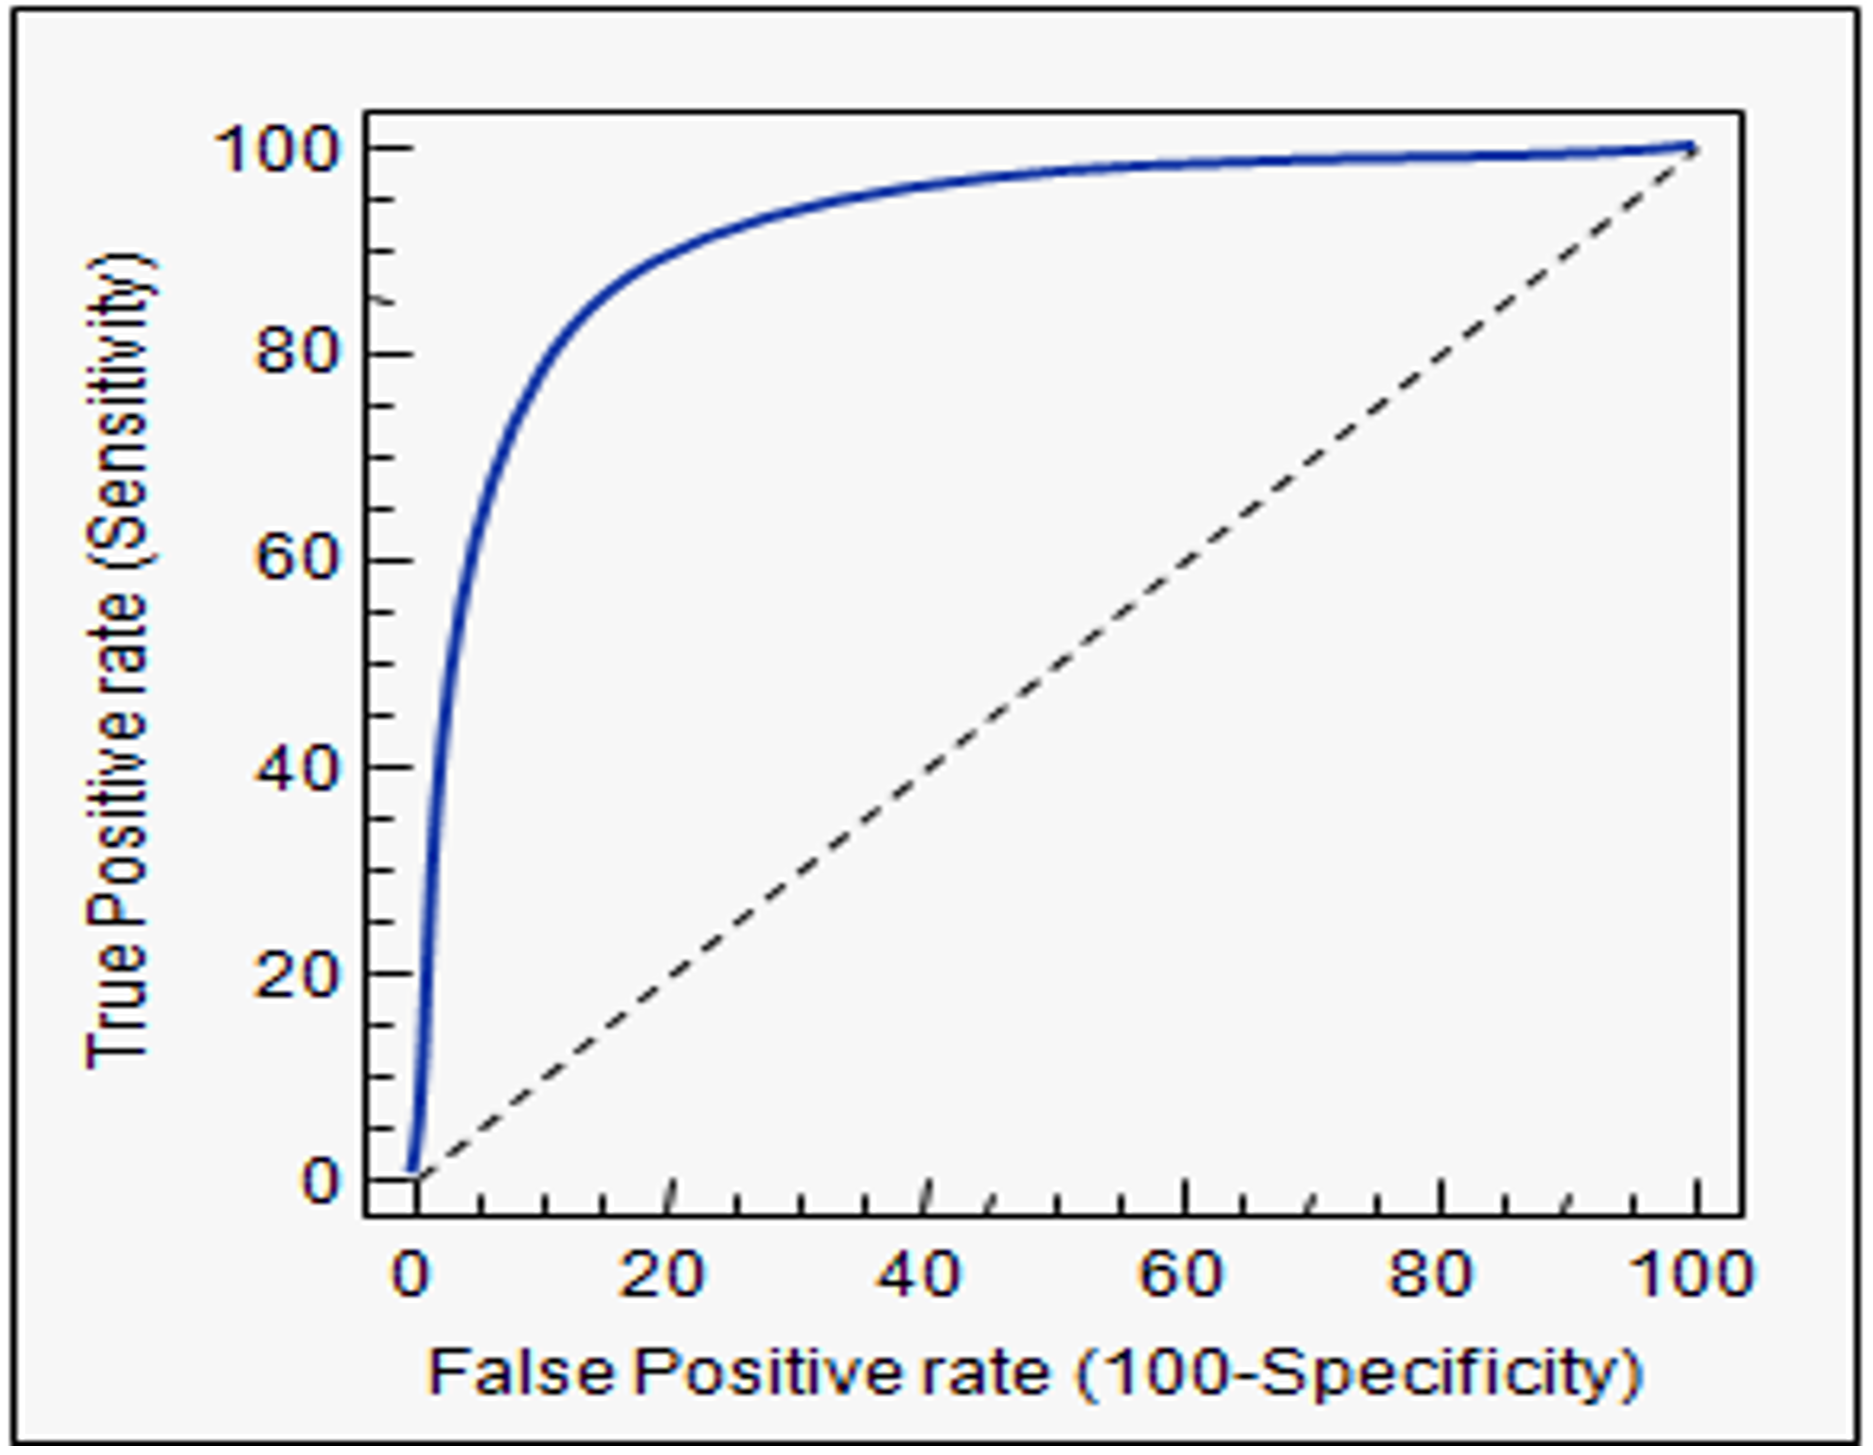
\includegraphics[width=0.47\textwidth]{Grafiken/ROC}
			%\caption{}
			\label{fig:ROC}
		\end{figure}
	
	AUC (area under curve) indicates model goodness, 1 being a perfect model 
	and below 0.5 (yellow line) a useless model (worse then a coin flip).
	
	
\end{frame}



\begin{frame}[fragile]{Classification: Boston housing data}
We investigate classification accuracy from a model for the median value of a home above \$ 30.000: Training and validation.
\begin{lstlisting}
> # Run logit model: Median value 0/1 ~ LowerPopul. + Number of rooms + Teacher/Pupil ratio
> fit<-glm(CAT..MEDV~LSTAT+RM+PTRATIO,data=train,family = "binomial")
> summary(fit)
Coefficients:
            Estimate Std. Error z value Pr(>|z|)
(Intercept) -12.5173     5.3884  -2.323 0.020179 *
LSTAT        -0.4006     0.1186  -3.378 0.000730 ***
RM            3.5765     0.6994   5.113 3.16e-07 ***
PTRATIO      -0.5783     0.1531  -3.778 0.000158 ***
(Dispersion parameter for binomial family taken to be 1)

Null deviance: 347.03  on 405  degrees of freedom
Residual deviance: 101.51  on 402  degrees of freedom
AIC: 109.51
\end{lstlisting}
\end{frame}


\begin{frame}[fragile]{Classification: Boston housing data}
	The \code{confusionMatrix()}-command returns the classification matrix.
	\begin{lstlisting}
	> # Create predictions - training vs. validation set 
	pred_t<-predict(fit,newdata = train,type = "response")
	pred_v<-predict(fit,newdata = vali,type = "response")	
	> # Evaluate performance - training vs. validation set 
	>  # Training - logit model
	confusionMatrix(ifelse(pred_t>0.5,1,0), train$CAT..MEDV)
	Reference
	Prediction   0   1
	0 338   8
	1   6  54          Accuracy : 0.9655
	>   # Validation - logit model
	confusionMatrix(ifelse(pred_v>0.5,1,0), vali$CAT..MEDV)
	Reference
	Prediction  0  1
	0 76  6
	1  2 16          Accuracy : 0.92
	\end{lstlisting}
\end{frame}



\begin{frame}[fragile]{Classification: Boston housing data}
We focus on the the validation set under the model and the naive methods.
	\begin{lstlisting}
	
> # Naive benchmark: the average
> y_fit_naive<-median(train$CAT..MEDV)

> # Create predictions
> pred_v_reg<-predict(fit,newdata = vali,type = "response")
> pred_v_naiv<-rep(y_fit_naive,length(vali$MEDV))

	\end{lstlisting}
\end{frame}


\begin{frame}[fragile]{Classification: Boston housing data}
We compare the confusion matrices.
	\begin{lstlisting}
	
> # Evaluate performance - validation set

> # Validation - logit model vs naive benchmark
> confusionMatrix(as.factor(ifelse(pred_v_reg > 0.5, 1, 0)), as.factor(vali$CAT..MEDV))
          Reference
Prediction  0  1
0 83  3
1  2 12

> confusionMatrix(as.factor(ifelse(pred_v_naiv > 0.5, 1, 0)), as.factor(vali$CAT..MEDV))
          Reference
Prediction  0  1
0 85 15
1  0  0
	
	\end{lstlisting}
\end{frame}


\begin{frame}[fragile]{Classification: Boston housing data}
We check the overall classification accuracy. 
	\begin{lstlisting}	
> predicted.classes <- as.factor(ifelse(pred_v_reg > 0.5, 1, 0))
> observed.classes <- as.factor(vali$CAT..MEDV)
> # Estimated accuracy - logit model 
> accuracy <- mean(observed.classes == predicted.classes)
0.95
> # Estimated missclassification rate - logit model 
> error <- mean(observed.classes != predicted.classes)
0.05

> # Confusion matrix, proportion of cases - logit model 
> table(observed.classes, predicted.classes) %>% 
prop.table() %>% round(digits = 3)
                predicted.classes
observed.classes    0    1
0 0.83 0.02
1 0.03 0.12
	
	\end{lstlisting}
\end{frame}

\begin{frame}[fragile]{Classification: Boston housing data}
We check the graphical representation of logits´accuracy. 
	\begin{lstlisting}
	> # Compute the eceiver operating characteristics curve (roc) - logit model 
> res.roc <- roc(observed.classes, pred_v_reg)
> plot.roc(res.roc, print.auc = TRUE)
	
	\end{lstlisting}
	
\begin{center}
	\includegraphics[width=0.8\textwidth]{bilder/roc}
\end{center}	
\end{frame}



\subsection{Cross-validation}

\begin{frame}
	\begin{center}
		\Large{\textcolor{dkblue}{Cross-validation}}
	\end{center}
\end{frame}



\begin{frame}
	\frametitle{Cross-validation (CV) as an evaluation method}

	\vspace*{0.5cm}
	\begin{itemize}
		\item \textbf{Problem}: parameters of a prediction are learned and tested on the same data $\rightarrow$ \textbf{Overfitting} - model memorizes training data but fails to predict unseen data
		\vspace{0.2cm}
		\item \textbf{General idea}: 
		\begin{enumerate}
			\item split data set into training set and testing set
			\vspace{0.2cm}
			\item fit model using training set only
			\vspace{0.2cm}
			\item use model to predict values of the testing set
			\vspace{0.2cm}
			\item use errors between prediction and actual value for evaluation 
		\end{enumerate}
		\item \textbf{Improvement (k-fold CV)}: divide data set into $k$ subsets and repeat the steps $k$ times $\rightarrow$ $k-1$ subsets are used as training sets and one subset as testing set, error is the average error across all $k$ trials 
		
	\end{itemize}
\end{frame}



\begin{frame}
	\frametitle{k-fold Cross-validation}
	\begin{columns}
		\begin{column}{7cm}
			\only<1>{\begin{figure}
					\includegraphics[width=7cm]{Grafiken/cv_first}
			\end{figure}}
			\only<2>{\begin{figure}
					\includegraphics[width=7cm]{Grafiken/cv_second}		
			\end{figure}}
			\only<3>{\begin{figure}
					\includegraphics[width=7cm]{Grafiken/cv_third}		
			\end{figure}}
			\only<4>{\begin{figure}
					\includegraphics[width=7cm]{Grafiken/cv_fourth}		
			\end{figure}}
			\only<5>{\begin{figure}
					\includegraphics[width=7cm]{Grafiken/cv_fourth_with}		
			\end{figure}}
		\end{column}
		\begin{column}{5cm}
			\begin{enumerate}[<+->]
				\item Divide data set randomly into $k$ subsets, here $k=3$
				\item Train using the gray and green points and test for the blue
				\item Train using the blue and green points and test for the grey
				\item Train using the blue and gray points and test for the green
				\item Use errors between prediction and actual value for evaluation
			\end{enumerate}	

		\end{column}
	\end{columns}
	
	
\end{frame}



\begin{frame}{CV for misclassified observations}
\begin{itemize}
  \item So far, we used CV in the
regression setting where the outcome is quantitative, and so have used
$MSE$ to quantify test error.
\vspace{0.2cm}
  \item When the outcome is categorical, CV works as described earlier, except that rather than using $MSE$ to quantify test error, we instead use the number
of misclassified observations.
\vspace{0.2cm}
\item LOOCV error rate $$ CV_{(n)}=\frac{1}{n}\sum_{i=1}^n I(y_i\neq \hat{y}_i).$$
\vspace{0.2cm}
\item The $k$-fold CV error rate and validation set error
rates are defined analogously.
\end{itemize}
\end{frame}

\begin{frame}[fragile]{Cross-validation: Boston housing data}
	Cross-validation can be automatically computed for any generalized linear model using the \code{cv.glm()}-command.
	\begin{lstlisting}
		> # Run linear regression model: Median value ~ Crime rate + Number of rooms + Teacher/Pupil ratio
		> fit<-glm(MEDV~CRIM+RM+PTRATIO,data=Daten)
		
		> # Leave-one-out cross-validation
		> cv_one_err<-cv.glm(Daten,fit)
		> cv_one_err$delta
		[1] 35.00064 34.99989
		
		> # 5-fold cross-validation
		> cv_5_err<-cv.glm(Daten,fit,K=5)
		> cv_5_err$delta
		[1] 34.98018 34.89865
	\end{lstlisting}
\end{frame}

\begin{frame}[fragile]{Cross-validation: Boston housing data}
	We investigate prediction error metrics from a model for the median value of a home: Linear vs. polynomial model for variable \textit{Crime rate}.
	\begin{lstlisting}
		> cv_error<-NULL
		>
		> for(i in 1:6){
			+   fit_poly<-glm(MEDV~poly(CRIM,degree=i)+RM+PTRATIO,data=Daten)
			+   cv_error[i]<-cv.glm(Daten,fit_poly,K=10)$delta[1]
			+ }
		> cv_error
		[1] 34.708 34.813 35.076 34.423 41.874 51.530
	\end{lstlisting}
	The results don't show a clear improvement from using higher-order ($>4$) polynomials. However, results may depend on the random split. 
\end{frame}

\begin{frame}[fragile]{Cross-validation: Boston housing data}
	\begin{center}
		\includegraphics[width=0.9\textwidth]{Grafiken/Error_CV}
	\end{center}
	Each CV approach was run 100 separate times, each with a different random split of the data into $K$ parts. The figure shows the median prediction error over replications.
\end{frame}



\subsection{Tree-based methods: Decision trees}

\begin{frame}
	\begin{center}
		\Large{\textcolor{dkblue}{Tree-based methods: Decision trees}}
	\end{center}
\end{frame}





\begin{frame}\frametitle{Prediction and classification approaches - A short overview}
	\begin{itemize}
	  \item Linear regression, logistic regression and multinomial logistic regression are common methods for prediction and classification.
	  	\vspace*{0.2cm}
	  \item These methods relate a response
variable to a set of explanatory variables - parametric nature.
\vspace*{0.2cm}
\item Linear relationships are being considered, which
means that the effect on the response of a change in the explanatory variable from
$x$ to $x+1$ is the same for any value $x$.
\vspace*{0.2cm}
\item With regression/classification trees, the models become truly nonparametric and they allow for very flexible representations.
	\end{itemize}
\end{frame}

\begin{frame}\frametitle{Tree-based methods: Regression/classification trees}
	\begin{itemize}
	  \item Here we describe tree-based methods for regression and
classification.
\vspace*{0.2cm}
\item These involve stratifying or segmenting the predictor space
into a number of simple regions.
\vspace*{0.2cm}
\item Since the set of splitting rules used to segment the
predictor space can be summarized in a tree, these types of
approaches are known as decision-tree methods.
\vspace*{0.2cm}
\item Decision trees can be applied to both regression and
classification problems.
	\end{itemize}
\end{frame}

\begin{frame}\frametitle{Pros and Cons: Regression/classification trees}
	\begin{itemize}
	  \item[+] Tree-based methods are simple and useful for
interpretation.
\vspace*{0.2cm}
	  \item[-] However they typically are not competitive with the best
supervised learning approaches in terms of prediction
accuracy.
\vspace*{0.2cm}
\item[+] Hence we also discuss bagging, random forests (and
boosting). These methods grow multiple trees which are
then combined to yield a single consensus prediction.
\vspace*{0.2cm}
\item[+/-] Combining a large number of trees can often result in
dramatic improvements in prediction accuracy, at the
expense of some loss interpretation.
	\end{itemize}
\end{frame}

\subsection{An introductory example}
\begin{frame}\frametitle{Predicting baseball players' salaries using regression trees}
In order to motivate regression trees, we begin with a simple example.\\
Example:\\
\vspace*{0.2cm}
	\begin{itemize}
	  \item We use the \textit{Hitters} data set (R-package: ISLR) to predict a baseball player's salary based on
the variable \textit{years} and
\textit{hits}.
\vspace*{0.2cm}
\item Years is the number of years that he has played in the major leagues.
\vspace*{0.2cm}
\item Hits is the number of hits that he made in the previous year.
\vspace*{0.2cm}
\item We log-transform salary so
that its distribution has a more symmetric shape (salary is measured in thousands of dollars).
	\end{itemize}
\end{frame}


\begin{frame}\frametitle{Predicting baseball players' salaries using regression trees}
How would you stratify the data?
\begin{figure}
		\centering
		\hspace*{-1.3cm}
		\includegraphics[width=0.65\textwidth]{Grafiken/GrafikBaseball} \\
Salary is color-coded from low (blue, green) to high (yellow, red)
	\end{figure}
\end{frame}

\begin{frame}\frametitle{Predicting baseball players' salaries using regression trees}
How would you stratify the data?
\begin{figure}
		\centering
		\hspace*{-1.3cm}
		\includegraphics[width=0.6\textwidth]{Grafiken/8_1}
	\end{figure}
\end{frame}

\begin{frame}\frametitle{Predicting baseball players' salaries using regression trees}
	\begin{itemize}
	  \item A regression tree for predicting the log
salary based on the number of years (played in the major leagues) and the number of hits (made in the previous year).
\vspace*{0.2cm}
\item At a given internal node, the label (of the form $X_j < t_k$)
indicates the left-hand branch emanating from that split, and
the right-hand branch corresponds to $X_j \geq t_k$. \item The
split at the top of the tree results in two large branches. The
left-hand branch corresponds to $Years<4.5$, and the right-hand
branch corresponds to $Years\geq 4.5$.
\vspace*{0.2cm}
\item The tree has two internal nodes (each decision defines a node) and three leaves/ terminal nodes. The number in each leaf is the mean of the response for
the observations that fall there.
	\end{itemize}
\end{frame}

\begin{frame}\frametitle{Predicting baseball players' salaries using regression trees}
Overall, the tree stratifies or segments the players into
three regions (terminal nodes or leaves) of predictor space:
\begin{figure}
		\centering
		\hspace*{-1.3cm}
		\includegraphics[width=0.57\textwidth]{Grafiken/8_2}
	\end{figure}
$R_1=\{X|Years < 4.5\}$, $R_2=\{X|Years\geq 4.5, Hits< 117.5\}$,\\$R_3=\{X|Years\geq 4.5, Hits\geq 117.5\}$
\end{frame}

\begin{frame}\frametitle{Terminology for trees}
	\begin{itemize}
	  \item In keeping with the tree analogy, the regions $R_1$, $R_2$, and
$R_3$ are known as \textit{terminal nodes}.
\vspace*{0.2cm}
\item Decision trees are typically drawn upside down, in the
sense that the leaves are at the bottom of the tree.
\vspace*{0.2cm}
\item The points along the tree where the predictor space is split
are referred to as \textit{internal nodes}.
\vspace*{0.2cm}
\item In the hitters tree, the two internal nodes are indicated by
the text $Years<4.5$ and $Hits<117.5$.
	\end{itemize}
\end{frame}


\begin{frame}\frametitle{Interpretation of results}
	\begin{itemize}
	  \item \textit{Years} is the most important factor in determining \textit{Salary},
and players with less experience earn lower salaries than
more experienced players.
\vspace*{0.2cm}
\item Given that a player is less experienced, the number of \textit{Hits}
that he made in the previous year seems to play little role
in his \textit{Salary}.
\vspace*{0.2cm}
\item Among players who have been in the major leagues for
five or more years, the number of \textit{Hits} made in the
previous year does affect \textit{Salary}, and players who made
more \textit{Hits} last year tend to have higher salaries.
\vspace*{0.2cm}
\item Surely an over-simplification, but compared to a regression
model, it is easy to display, interpret and explain.
	\end{itemize}
\end{frame}






\subsubsection{Regression trees}



\begin{frame}
	\begin{center}
		\Large{\textcolor{dkblue}{Regression trees}}
	\end{center}
\end{frame}


\begin{frame}\frametitle{Building regression trees: Segmentation of the space}
The process of building a regression tree consists of mainly two steps:
\vspace*{0.2cm}
	\begin{enumerate}
	  \item We divide the predictor space - that is, the set of possible values for
$X_1,X_2,...,X_p$ - into $J$ distinct and non-overlapping regions,
$R_1,R_2,...,R_J$.
\vspace*{0.2cm}
\item For every observation that falls into the region $R_j$, we make the same
prediction, which is simply the mean of the response values for the
training observations in $R_j$.
	\end{enumerate}
\vspace*{0.2cm}
Comment to step 1): The regions could have any shape. However, we
choose to divide the predictor space into high-dimensional
rectangles, or boxes, for simplicity and for ease of
interpretation of the resulting predictive model.
\end{frame}

\begin{frame}\frametitle{Building regression trees: Segmentation of the space}
How should we divide the predictor space?\\
The goal is to find boxes $R_1,R_2,...,R_J$ that minimize residual sum of squares
$$RSS=\sum_{j=1}^J\sum_{i\in R_j}\left(y_i-\hat{y}_{R_j}\right)^2,$$
where $\hat{y}_{R_j}$ is the mean response for the training observations within $R_j$.
\begin{itemize}
\item Unfortunately, it is computationally infeasible to consider
every possible partition of the feature space into $J$ boxes.
\vspace*{0.2cm}
\item For this reason, we take a top-down approach that
is known as recursive binary splitting.
\vspace*{0.2cm}
\item The best split is made at that particular step,
rather than looking ahead and picking a split that will lead
to a better tree in some future step.
\end{itemize}
\end{frame}

\begin{frame}\frametitle{Building regression trees: Segmentation of the space}
\begin{itemize}
\item We first select (both) the predictor $X_j$ and the cutpoint $s$ such
that splitting the predictor space into the regions
$R_1(j,s)=\{X|X_j<s\}$ and $R_2(j,s)=\{X|X_j\geq s\}$ leads to the greatest possible
reduction in $RSS$.
\item We minimize the equation:
$$\min_{j,s}\left[\sum_{i: x_i\in R_1(j,s)}\left(y_i-\hat{y}_{R_1}\right)^2+\sum_{i: x_i\in R_2(j,s)}\left(y_i-\hat{y}_{R_2}\right)^2\right]$$
\item Next, we repeat the process, looking for the best $X_j$ and cutpoint $s$ to split the data further to
minimize the $RSS$ within each of the resulting regions. We split one of the two previously identified regions. We now have three regions.
\end{itemize}
\end{frame}

\begin{frame}\frametitle{Building regression trees: Segmentation of the space}

\begin{itemize}
\item We split one of these three regions further to minimize the $RSS$.
\vspace*{0.2cm}
\item The process continues until a
stopping criterion is reached; for instance, we may continue
until no region contains more than five observations.
\vspace*{0.2cm}
\end{itemize}
\textbf{Prediction}\\
We predict the response for a given test (validation) observation using
the mean of the training observations in the region to
which that test observation belongs.
\end{frame}

\begin{frame}\frametitle{Tree Pruning}

\begin{itemize}
\item The process described above may produce good predictions on the training
set, but is likely to overfit the data, leading to poor test (validation) set performance.
\vspace*{0.2cm}
\item A smaller tree with fewer splits (that is, fewer regions
$R_1,...,R_J$) might lead to lower variance and better
interpretation at the cost of a little bias.
\vspace*{0.2cm}
\item One strategy is to grow a very large tree $T_0$, and then
prune it back in order to obtain a subtree - \textit{Cost complexity pruning}.
\end{itemize}
\end{frame}

\begin{frame}\frametitle{Tree Pruning - Cost complexity pruning}
For each value of $\alpha$ there corresponds a subtree $T\subset T_0$ such that
$$\sum_{m=1}^{|T|}\sum_{i: x_i\in R_m}\left(y_i-\hat{y}_{R_m}\right)^2+\alpha |T|$$ is as small as possible.
\begin{itemize}
\item $|T|$ indicates the number of leaves/ terminal nodes.
\item The tuning parameter $\alpha$ controls a trade-off between the
subtree's complexity and its fit to the training data.
\item When $\alpha=0$, then the subtree $T$
will simply equal $T_0$, the formula just measures the training error.
\item As $\alpha$ increases, there is a price to pay for having a tree with
many terminal nodes.
\item We select an optimal value $\hat{\alpha}$ using cross-validation.
\item We then return to the full data set and obtain the subtree
corresponding to $\hat{\alpha}$.
\end{itemize}
\end{frame}

\begin{frame}\frametitle{Summary: Constructing a regression tree}
\begin{enumerate}
\item Use recursive binary splitting to grow a large tree on the training
data, stopping only when each terminal node has fewer than some
minimum number of observations.
\vspace*{0.2cm}
\item Apply cost complexity pruning to the large tree in order to obtain a
sequence of best subtrees, as a function of $\alpha$.
\vspace*{0.2cm}
\item Use $K$-fold cross-validation to choose $\alpha$. That is, divide the training
observations into $K$ folds. For each $k=1,...,K$:
\begin{itemize}
  \item[-] Build a regression tree (for a given $\alpha$) on all $K-1$th folds of the training data.
  \item[-] Evaluate the mean squared prediction error on the data in the
left-out $k$th fold, as a function of $\alpha$.
\end{itemize}
\vspace*{0.2cm}
Average the results for each value of $\alpha$, and pick $\alpha$ to minimize the
average error.
\vspace*{0.2cm}
\item Return the subtree from Step 2 that corresponds to the chosen value
of $\alpha$.
\end{enumerate}
\end{frame}





\subsubsection{Prediction and classification trees}

\begin{frame}
	\begin{center}
		\Large{\textcolor{dkblue}{Prediction and classification methods: Example in R  }}
	\end{center}
\end{frame}


\begin{frame}[fragile]{Regression trees in R: Boston housing data}
The \code{rpart()}-command constructs a regression tree and returns the results as an object.

\begin{lstlisting}
# Loading libraries and the data
library(rpart)
library(partykit)

# Run a regression tree using the rpart command
fit<-rpart(formula, data, method, minsplit, cp, subset)
\end{lstlisting}
\begin{itemize}
  \item \code{minsplit} specifies min. number of units that must exist in a node in order for a split to be attempted.
  \item \code{cp} defines the complexity parameter $\alpha$ in the pruning of the tree.
   \item \code{subset} specifies the units in the training data set from the available data.
\end{itemize}
\end{frame}

\begin{frame}[fragile]{Regression trees in R: Boston housing data}
Grow a general regression tree with\\
Crime rate + River 1/0 + Number of rooms + Teacher/Pupil ratio

\begin{lstlisting}
# Change complexity parameter alpha to 0 - full tree
> fit<-rpart(MEDV~CRIM+CHAS+RM+PTRATIO, data=Daten, minsplit=10, cp=0, subset=inTrain)
# Display the results of cross-validation
> printcp(fit)
Variables actually used in tree construction:
[1] CHAS    CRIM    PTRATIO RM
Root node error: 34771/406 = 85.643
           CP nsplit rel error  xerror     xstd
1  0.45424798      0   1.00000 1.00491 0.092344
2  0.10154523      1   0.54575 0.59452 0.063519
3  0.09118098      2   0.44421 0.50018 0.070210
.  ..........      .   ....... ....... ........
57 0.00014848     74   0.13146 0.43197 0.075392
58 0.00013117     75   0.13131 0.43179 0.075389
59 0.00000000     76   0.13118 0.43207 0.075387
\end{lstlisting}
\end{frame}

\begin{frame}[fragile]{Regression trees in R: Boston housing data}
The \code{prune()}-command prunes the regression tree. The tree can be visualized by \code{plot()}-command.

\begin{lstlisting}
> # Visualize cross-validation results
> plotcp(fit)
>
> # Prune the tree
> fit$cptable[which.min(fit$cptable[,"xerror"]),"CP"]
[1] 0.02605373
> pfit<- prune(fit, cp=0.02605373) # from cptable
>
> # Plot the pruned regression tree
> plot(as.party(pfit))
\end{lstlisting}
\end{frame}

\begin{frame}
\frametitle{Regression trees in R: Boston housing data}
\begin{center}
\includegraphics[width=0.95\textwidth]{Grafiken/Regtree_plot}
\end{center}
\end{frame}

\begin{frame}[fragile]{Regression trees in R: Boston housing data}
Compare the performance of the pruned tree with the full tree on the validation data.
\begin{lstlisting}
# Predictions for the validation data
> pred_v_tree<-predict(fit,newdata=vali)
> pred_v_ptree<-predict(pfit,newdata=vali)

# Evaluate performance
> accuracy(pred_v_tree,vali$MEDV)
              ME   RMSE   MAE    MPE    MAPE
Test set -0.6629 5.8775 4.001 -9.270 21.3263
> accuracy(pred_v_ptree,vali$MEDV)
              ME   RMSE   MAE    MPE    MAPE
Test set -0.6485 5.6786 3.881 -9.676 20.3017
\end{lstlisting}
\end{frame}

\subsection{Classification trees}


\begin{frame}
	\begin{center}
		\Large{\textcolor{dkblue}{Classification trees}}
	\end{center}
\end{frame}

\begin{frame}\frametitle{Classification trees - Some first comments}
\begin{itemize}
\item A \textbf{classification tree} is very similar to a regression tree, except that it is
classification
used to predict a \textbf{qualitative response }rather than a quantitative one.
\vspace*{0.2cm}
\item We predict that
each observation belongs to the most commonly occurring class of training
observations in the region to which it belongs.
\vspace*{0.2cm}
\item We are often interested not only in the \textbf{class prediction}
corresponding to a particular terminal node region, but also in the \textbf{class
proportions} among the training observations that fall into that region.
\end{itemize}
\end{frame}

\begin{frame}\frametitle{Building classification trees}
\begin{itemize}
\item We use recursive
binary \textbf{splitting} to grow a classification tree.
\vspace*{0.2cm}
\item In the classification setting, $RSS$ cannot be used as a
criterion for making the binary splits.
\vspace*{0.2cm}
\item A natural alternative to $RSS$ is the classification error rate:
$$E=1-\max_k(\hat{p}_{mk}),$$ where $\hat{p}_{mk}$ represents the proportion of training observations in the $m$-th
region that are from the $k$-th class.
\vspace*{0.2cm}
\item The \textbf{classification error rate} is
simply the fraction of the training observations in that region that do not
belong to the most common class.
\end{itemize}
\end{frame}

\begin{frame}\frametitle{Building classification trees - Two other measures}
\begin{itemize}
\item The classification error is not sufficiently sensitive for
tree-growing.
\item The Gini index is defined by:
$$G=\sum_{k=1}^K\hat{p}_{mk}(1-\hat{p}_{mk})$$ and measures the variation across the $K$ classes (Gini is small when all $\hat{p}_{mk}$ are close to
zero or one).
\item Gini index is a measure of
\textit{node purity} - a small value indicates that a node contains
predominantly observations from a single class.
\item An alternative to the Gini index is cross-entropy
$$D=-\sum_{k=1}^K\underbrace{\hat{p}_{mk}\log(\hat{p}_{mk})}_{\leq 0}.$$
\item The cross-entropy takes a value near zero if the $\hat{p}_{mk}$ are all near
zero or near one (small values indicate that nodes are pure).
\end{itemize}
\end{frame}


\begin{frame}
	\frametitle{When to Stop}
	If tree growing is never stopped, it can result in perfectly pure nodes of 
	one observation each. This is likely to overfit the training data and give 
	poor prediction on the test set. 
	
	\vspace{0.3cm}
	
	Strategy to overcome too complex models:
	\begin{itemize}
		\item stop if decrease in impurity is smaller than a threshold
		\item grow a very large tree and prune it back ('cut branches')
	\end{itemize}
\end{frame}


\begin{frame}[fragile]{Classification trees in R: Boston housing data}
Classification trees can be fitted by using the same commands.
\begin{lstlisting}
# Run a classification tree using the rpart command
> fit<-rpart(MEDV_Fac~CRIM+CHAS+RM+PTRATIO, data=Daten, method="class", minsplit=5, cp=0, subset=inTrain)

> # Prune the tree
> fit$cptable[which.min(fit$cptable[,"xerror"]),"CP"]
[1] 0.03225806
> pfit<- prune(fit, cp=0.03225806) # from cptable

> # Plot the pruned classification tree
> plot(as.party(pfit))
\end{lstlisting}
\end{frame}

\begin{frame}
\frametitle{Classification trees in R: Boston housing data}
\begin{center}
\includegraphics[width=0.95\textwidth]{Grafiken/Classtree_plot}
\end{center}
\end{frame}

\begin{frame}[fragile]{Classification trees in R: Boston housing data}
Compare the performance of the pruned tree with the full tree on the validation data.
\begin{lstlisting}
# Predictions for the validation data
> pred_v_tree<-predict(fit,newdata=vali,type="class")
> pred_v_ptree<-predict(pfit,newdata=vali,type="class")

# Evaluate performance
> confusionMatrix(pred_v_tree, vali$MEDV_Fac)
Prediction Below Above
     Below   120     6
     Above     8    16
               Accuracy : 0.9067
> confusionMatrix(pred_v_ptree, vali$MEDV_Fac)
Prediction Below Above
     Below   122     3
     Above     6    19
               Accuracy : 0.94
\end{lstlisting}
\end{frame}

\begin{frame}\frametitle{Advantages and disadvantages of trees}
\begin{itemize}
\item[+] Trees are very easy to explain to people.
\vspace*{0.2cm}
\item[+] Some people believe that decision trees more closely mirror
human decision-making than do the regression and
classification approaches.
\vspace*{0.2cm}
\item[+] Trees can be displayed graphically, and are easily
interpreted even by a non-expert (especially if they are
small).
\vspace*{0.2cm}
\item[-] Trees generally do not have the same level of
predictive accuracy as some of the other regression and
classification approaches.
\vspace*{0.2cm}
\item[-] The decision trees suffer from high variance.
\end{itemize}
\vspace*{0.2cm}
However, by aggregating many decision trees, the predictive
performance of trees can be substantially improved.
\end{frame}


\end{document} 